%versi 2 (8-10-2016)
\lstset{
  basicstyle=\ttfamily,
  columns=fullflexible,
  frame=single,
  breaklines=true,
  showlines=true,
  postbreak=\mbox{\textcolor{red}{$\hookrightarrow$}\space},
}

\chapter{Landasan Teori}
\label{chap:teori}
\setcounter{secnumdepth}{3}
%Pada bab ini dijelaskan dasar-dasar teori mengenai \textit{BlueTape}, \textit{Heroku}, \textit{PostgreSQL}, \textit{GMail}, dan \textit{Line@}.



%2.1 BlueTape
\section{\textit{BlueTape}}
\label{sec:BlueTape}
\textit{BlueTape} adalah perangkat lunak yang berfungsi untuk membantu urusan-urusan \textit{paper-based} di FTIS UNPAR menjadi \textit{paperless}. Perangkat lunak ini berbasis web dengan memanfaatkan \textit{CodeIgniter} dan \textit{ZURB Foundation}. Saat ini aplikasi ini memiliki dua layanan, yaitu Transkrip \textit{Request} / \textit{Manage} dan Perubahan Kuliah \textit{Request} / \textit{Manage}. Layanan Transkrip \textit{Request} / \textit{Manage} memberikan layanan untuk melakukan permohonan serta pencetakan transkrip mahasiswa. Sedangkan layanan Perubahan Kuliah \textit{Request} / \textit{Manage} memberikan layanan untuk permohonan dan pencetakan perubahan jadwal kuliah oleh dosen. \footnotemark
\footnotetext{https://github.com/ftisunpar/BlueTape}



%2.2 Heroku
\section{Heroku ~\cite{heroku}}
\label{sec:Heroku}
Heroku adalah \textit{platform cloud} yang memungkinkan pengembang untuk membangun, menjalankan, dan mengoperasikan perangkat lunak pada \textit{cloud}. Heroku mendukung beberapa bahasa pemrograman, meliputi : Ruby, Node.js, Java, Python, Clojure, Scala, Go, dan PHP. 

\subsection{Arsitektur Heroku}
Heroku memungkinkan seorang pengembang untuk menyebarkan (\textit{deploy}), menjalankan (\textit{run}), dan mengelola (\textit{manage}) perangkat lunak yang ditulis di dalam bahasa Ruby, Node.js, Java, Python, Clojure, Scala, Go, dan PHP. Heroku mendefinisikan perangkat lunak sebagai gabungan dari \textit{source code} yang ditulis di dalam salah satu bahasa ini (dapat berupa \textit{framework}), deskripsi dependensi yang dipakai, dan Procfile (jika diperlukan).

\subsubsection{Dependensi}
Pengembang perlu mendeskripsikan dependensi tambahan yang diperlukan agar perangkat lunak dapat dibangun dan dijalankan. Aturan penulisan deskripsi dependensi berbeda-beda untuk tiap bahasa. Contohnya pada bahasa Ruby deskripsi dependensi dituliskan dalam dokumen \texttt{Gemfile}, pada bahasa Python ditulis di dokumen \texttt{requirements.txt}, pada bahasa Node.js ditulis di dokumen \texttt{package.json}, pada bahasa Java ditulis di dokumen \texttt{pom.xml}, dan seterusnya.

\subsubsection{Tipe Proses (Proccess Type)}
Di dalam perangkat lunak web, terdapat dua atau lebih titik masuk. Itu artinya ada dua atau lebih perintah untuk menjalankan perangkat lunak. Setiap titik masuk ini disebut tipe proses (\texttt{process type}). Tipe proses berbeda untuk tiap perangkat lunak.

Tipe proses dapat berupa web server dari perangkat lunak, berbagai tipe \textit{worker process}, \textit{singleton process} (contoh : clock), dan tugas yang harus dijalankan sebelum sebuah release disebar. Di antara beragam tipe proses tersebut, ada dua tipe proses spesial : tipe proses \texttt{web} dan \texttt{release}. Tipe proses \texttt{web} adalah satu-satunya tipe proses yang dapat menerima arus HTTP eksternal dari router Heroku. Jika sebuah perangkat lunak melibatkan web server, pengembang harus menyatakannya sebagai proses \texttt{web}. Tipe proses \texttt{release} adalah tipe proses yang digunakan untuk menyebutkan perintah yang dijalankan selama fase release.

Tipe proses dan dyno saling berhubungan. Tipe proses adalah prototipe yang menjadi tempat dimana dyno dibentuk. Semakin banyak dyno pada suatu tipe proses maka konkurensi untuk pekerjaan yang ditangani tipe proses tersebut akan meningkat. Semakin banyak tipe proses maka semakin beragam beban kerja.

Setiap tipe proses memiliki spesialisasinya sediri pada jenis pekerjaan tertentu. Misalnya, sebuah perangkat lunak memiliki dua jenis pekerja : pekerja untuk pekerjaan yang mendesak dan pekerja untuk pekerjaan yang berlangsung dengan lama. Dengan melakukan pembagian seperti itu, pekerjaan yang mendesak lebih cepat tertangani. Selain itu, penggunaan sumber daya lebih mudah dikontrol dan dikalkulasi.

Untuk mengatur berapa banyak dyno yang bekerja di suatu proses, perintah yang dibutuhkan adalah \texttt{heroku ps:scale} diikuti dengan daftar pasangan tipe proses dengan jumlah dyno yang ditugaskan untuk proses tersebut. Contoh :
\begin{lstlisting}

	heroku ps:scale web=2 worker=4 clock=1
	
\end{lstlisting}

Selain dapat mengatur jumlah dyno yang ditugaskan pada suatu pekerjaan, jangka waktu pekerjaan itu dilakukan juga dapat diatur. Caranya dengan menggunakan add-on Heroku Scheduler atau menggunakan tipe proses khusus untuk mengatur jadwal pekerjaan.

\subsubsection{Procfile}
Pengembang perlu memberitahu Heroku bagian perangkat lunak yang dapat dijalankan. Jika pengembang menggunakan framework yang sudah ada, Heroku dapat mencari tahu. Contohnya, di dalam Ruby pada Rails, biasanya \texttt{rails server}, di dalam Django adalah \texttt{python <app>/manage.py runserver} dan di dalam Node.js adalah \texttt{main} field di dalam \texttt{package.json}. Untuk perangkat lunak lain, pengembang mungkin perlu untuk secara eksplisit menyatakan apa yang harus dieksekusi. Caranya dengan menyertakan sebuah dokumen teks bernama Procfile. 

Dokumen Procfile tidak memiliki ekstensi dokumen, seperti \texttt{.txt}, \texttt{.docx}, \texttt{.jpg} dan lain-lain. Apabila Procfile diberi ekstensi dokumen (contoh : Procfile.txt), maka Procfile tersebut tidak sah. Selain itu, Procfile harus diletakkan di direktori root. Jika diletakkan di tempat lain, Procfile tidak akan berfungsi sebagaimana mestinya.

Isi dari Procfile adalah satu atau lebih baris yang menyatakan sebuah tipe proses. Format penulisan tiap baris Procfile adalah : 
\begin{lstlisting}

	<process type>: <command>

\end{lstlisting}
\texttt{<process type>} (tipe proses) adalah nama perintah yang mengandung huruf dan angka, seperti : \texttt{web}, \texttt{worker}, \texttt{urgentworker}, \texttt{clock}, dan lain-lain. Untuk perangkat lunak sederhana, pengembang cukup menuliskan tipe proses \texttt{web} saja. \texttt{<command>} adalah perintah yang setiap dyno dari tipe proses tersebut harus jalankan pada saat startup, seperti \texttt{rake jobs : work}. Contoh isi Procfile :
\begin{lstlisting}

	web: java -jar lib/foobar.jar \textdollar PORT

\end{lstlisting}
Pada contoh, \texttt{web} merupakan \texttt{<process type>}, sedangkan \texttt{web: java -jar lib/foobar.jar \textdollar PORT} adalah perintah yang harus dijalankan pada saat startup.

Heroku adalah polyglot platform : Heroku memungkinkan Anda membangun, menjalankan, dan mengatur perangkat lunak di cara yang serupa dalam segala bahasa pemrograman - menggunakan dependensi dan Procfile. Procfile menyingkap aspek arsitektur dari perangkat lunak dan arsitektur ini memungkinkan pengembang, contohnya, mengatur setiap bagian secara independen. Namun, membuat Procfile tidak wajib untuk sebagian besar bahasa pemrograman yang didukung Heroku. Heroku akan secara otomatis mendeteksi bahasa yang digunakan, dan membuat tipe proses \texttt{web} untuk menjalankan server perangkat lunak. Apabila perangkat lunak menggunakan \texttt{heroku.yml} sebagai build manifest, Procfile juga tidak diwajibkan. Perintah yang disebutkan di bagian \texttt{run} pada \texttt{heroku.yml} harus mengikuti format yang sama dengan format Procfile.

\subsubsection{Deploy Perangkat Lunak}
Heroku menggunakan Git sebagai sarana  utama untuk melakukan deploy perangkat lunak. Deploy disini adalah proses penyebaran perangkat lunak dari satu lingkungan ke lingkungan lain, misalnya dari lingkungan mesin pengembang perangkat lunak ke lingkungan heroku. Sedangkan Git adalah sistem version control terdistribusi yang kuat yang digunakan banyak pengembang untuk mengelola dan menerjemahkan source code (https://git-scm.com/). Heroku juga menyediakan cara lain untuk melakukan deploy, seperti dengan menggunakan GitHub integration atau Heroku API.  

Ketika perangkat lunak baru dibuat di Heroku, Heroku secara otomatis membuat Git remote baru. Heroku secara otomatis menamainya \texttt{Heroku}, namun pengembang dapat menggantinya. Git remote ini terhubung dengan perangkat lunak tersebut dan berfungsi sebagai alamat yang digunakan saat melakukan deploy. Sehingga apabila pengembang ingin melakukan deploy, maka pengembang hanya perlu melakukan \texttt{git push} diikuti dengan nama remote dan nama branch repository. Contoh :
\begin{lstlisting}

	$ git push heroku master
	
\end{lstlisting}

\subsubsection{Membangun Perangkat Lunak}
Ketika platform Heroku menerima source code perangkat lunak, heroku akan memulai pembangunan (build) berdasarkan source code. Mekanisme build biasanya tergantung bahasa pemrograman yang dipakai, tapi mengikuti pola yang sama. Mekanisme build biasanya mengambil dependensi yang ditentukan, dan menciptakan aset yang diperlukan. Contohnya, perangkat lunak Java mungkin mengambil dependensi library biner menggunakan Maven, mengompilasinya, lalu menghasilkan dokumen JAR untuk dieksekusi.

Source code untuk perangkat lunak, dependensi yang diraih, dan hasil dari fase build digabungkan ke dalam slug. Slug adalah gabungan dari source code, dependensi yang diambil, language runtime, dan hasil kompilasi atau keluaran yang dihasilkan oleh sistem build yang siap untuk dieksekusi. Slug ini adalah aspek dasar dari eksekusi perangkat lunak. Slug berisi perangkat lunak yang sudah dikompilasi, digabungkan, dan siap untuk dijalankan.

Di belakang proses kompilasi slug terdapat buildpack. Buildpack mengambil perangkat lunak, dependensi, dan language runtime dan kemudian menghasilkan slug. Buildpack bersifat open source, sehingga memungkinkan pengembang memperluas Heroku ke bahasa pemrograman lain dan framework.

\subsubsection{Buildpack}
Buildpack bertanggung jawab untuk mengubah source code menjadi slug, sehingga dyno dapat mengeksekusinya. Buildpack terdiri dari sekumpulan script yang ditulis dalam bahasa pemrograman yang sama dengan source code. Script tersebut akan mengambil dependensi, mengeluarkan aset atau kode yang sudah dikompilasi, dan sebagainya. Keluaran ini akan digabungkan ke dalam slug oleh slug compiler.

% Gambar tabel buildpack (https://devcenter.heroku.com/articles/buildpacks)

Heroku akan mencari buildpack yang sesuai dan menggunakannya untuk mengompilasi perangkat lunak. Jika build sukses, buildpack yang sudah terdeteksi sesuai akan secara permanen diatur untuk push selanjutnya. Buildpack yang telah dimodifikasi dapat dipakai untuk mendukung bahasa atau framework yang tidak dapat di cakup oleh buildpack resmi.

Buildpack yang digunakan dapat diubah dengan mengatur nilai buildpack. Caranya dengan mengetikkan perintah ini pada command shell :
\begin{lstlisting}

	$ heroku buildpacks:set <nama buildpack>
	
\end{lstlisting}
<nama buildpack> adalah nama buildpack yang ingin dipakai, contoh : \texttt{heroku/php}. Buildpack baru akan digunakan saat push berikutnya. 

Apabila pengembang ingin mengatur buildpack yang dipakai saat perangkat lunak pertama kali dibuat, maka dapat menggunakan perintah ini :
\begin{lstlisting}

	$ heroku create myapp --buildpack <nama buildpack>
	
\end{lstlisting}
<nama buildpack> adalah nama buildpack yang ingin dipakai.

Buildpack juga dapat secara eksplisit diatur di dalam app.json sehingga perangkat lunak yang dibuat menggunakan tombol Heroku dapat menggunakan buildpack yang telah dimodifikasi.

Apabila pengembang ingin menghilangkan buildpack dari perangkat lunak, pengembang dapat mengetikkan perintah :
\begin{lstlisting}

	$ heroku buildpacks:remove <nama buildpack>
	
\end{lstlisting}
<nama buildpack> adalah nama buildpack yang ingin dipakai. Hal yang harus diperhatikan adalah jika buildpack tidak ada, maka proses mendeteksi buildpack yang sesuai akan dijalankan lagi saat push berikutnya.

Selain dapat menggunakan buildpack yang telah dimodifikasi, terdapat third-party buildpack tersedia di Element marketplace atau menggunakan CLI. Pada CLI, ketikkan perintah :
\begin{lstlisting}

	$ heroku buildpacks:search <kata kunci>
	
\end{lstlisting}
<kata kunci> misalnya adalah nama bahasa pemrograman yang dipakai, misalnya \texttt{elixir}. Apabila ingin melihat informasi tentang buildpack yang didapat, maka ketikkan perintah :
\begin{lstlisting}

	$ heroku buildpacks:info <kata kunci>
	
\end{lstlisting}
<nama buildpack> adalah nama buildpack yang ingin dipakai. Dengan perintah tersebut, informasi seperti deskripsi, kategori, lisensi, source, dan informasi lainnya dapat dilihat.

Apabila pengembang ingin mengembalikan perangkat lunak ke buildpack awalnya, maka pengembang dapat mengetikkan perintah :
\begin{lstlisting}

	$ heroku buildpacks:clear
	
\end{lstlisting}

Biasanya buildpack yang dipakai oleh perangkat lunak hanya satu, tapi ada beberapa kasus buildpack yang dipakai tidak cukup hanya satu. Beberapa kasus tersebut adalah :
\begin{itemize}
\item Menjalankan buildpack untuk tiap bahasa pemrograman yang perangkat lunak gunakan. Contohnya, menjalankan JavaScript buildpack untuk aset dan buildpack Ruby untuk perangkat lunak.
\item Menjalankan proses daemon seperti \texttt{pgbouncer} dengan perangkat lunak.
\item Menarik dependensi sistem dengan apt.
\end{itemize}

Pengembang dapat menentukan buildpack-buildpack yang diperlukan perangkat lunak dan mengatur urutan eksekusinya dengan Heroku CLI. Untuk menambahkan buildpack yang ingin dipakai, pengembang dapat mengetikkan perintah :
\begin{lstlisting}

	$ heroku buildpacks:add --index <index> <nama buildpack>

\end{lstlisting}
<index> adalah urutan eksekusi buildpack, sedangkan <nama buildpack> adalah nama buildpack yang ingin dipakai.

Untuk mengubah buildpack yang dipakai pada urutan eksekusi tertentu, pengembang dapat mengetikkan perintah :
\begin{lstlisting}

	$ heroku buildpacks:set --index <index> <nama buildpack>
	
\end{lstlisting}
<index> adalah urutan eksekusi buildpack, sedangkan <nama buildpack> adalah nama buildpack yang ingin dipakai.

Untuk melihat daftar buildpack yang dipakai oleh perangkat lunak, ketikkan perintah :
\begin{lstlisting}

	$ heroku buildpacks

\end{lstlisting}
Buildpack terakhir pada daftar adalah buildpack yang digunakan untuk menentukan tipe proses dari perangkat lunak. Tipe proses lain yang disebutkan akan diabaikan.

Untuk melihat daftar perintah yang dapat digunakan untuk mengatur buildpack, pengembang dapat mengetikkan perintah :
\begin{lstlisting}

	$ heroku help buildpacks

\end{lstlisting}

\subsubsection{Dyno}
Heroku mengeksekusi perangkat lunak dengan menjalankan perintah yang telah ditulis di dalam Procfile. Heroku akan menjalankan dyno yang telah dimuat dengan slug yang telah disiapkan. Dyno adalah wadah perangkat lunak berbasis Unix yang terisolasi, tervirtualisasi, dan menyediakan lingkungan yang dibutuhkan untuk menjalankan suatu perangkat lunak. Umumnya, jika perangkat lunak di-deploy ke Heroku untuk pertama kali, Heroku akan menjalankan satu web dyno secara otomatis.

Setiap dyno termasuk dalam salah satu dari konfigurasi berikut :
\begin{itemize}
\item Web : Web dyno adalah dyno dari tipe proses "web" yang disebutkan di dalam Procfile. Web dyno adalah satu-satunya dyno yang dapat menerima arus HTTP dari router Heroku.
\item Worker : Worker dyno adalah dyno dari tipe proses apapun selain "web" yang disebutkan di dalam Procfile. Worker dyno biasanya digunakan untuk pekerjaan di latar belakang, sistem antrian, dan pekerjaan yang memiliki jangka waktu.
\item One-off : One-off dyno adalah dyno yang bersifat sementara yang dapat berjalan terpisah atau dengan masukan/keluaran dari terminal lokal.
\end{itemize}. Dyno ini dapat digunakan untuk tugas yang bersifat administratif, seperti migrasi basis data dan sesi konsol. Dyno ini juga dapat digunakan untuk melakukan pekerjaan di latar belakang yang bersifat sesekali, seperti Heroku Scheduler.

Heroku menyediakan beberapa tipe dyno yang berbeda. Tiap dyno memiliki sifat yang unik dan kinerja yang berbeda. Untuk semua pengguna Heroku, tersedia pilihan dyno tipe Free, Hobby, Standard, dan Performance. Ada satu tipe dyno lagi, yaitu tipe Private. Dyno tipe Private hanya tersedia di Heroku Enterpise yang diperuntukkan untuk organisasi.

Dyno dapat diskala secara horizontal dan vertikal. Untuk menskala secara horizontal, tambahkan lebih banyak dyno. Contohnya, menambah web dyno agar dapat menangani arus yang lebih besar. Untuk menskala secara vertikal, gunakan dyno yang lebih besar. Dyno yang lebih besar berarti jumlah pemakaian memori RAM yang lebih besar. Jumlah RAM maksimal yang tersedia untuk perangkat lunak tergantung dari tipe dyno yang digunakan. Penskalaan secara horizontal dan vertikal ini adalah fitur dari dyno profesional, dan tidak tersedia untuk dyno tipe free dan hobby.

Perangkat lunak dengan banyak dyno yang berjalan akan memiliki resiko kegagalan yang lebih rendah daripada yang sedikit. Jika ada dyno yang hilang, perangkat lunak dapat terus memproses permintaan sementara dyno yang hilang diganti. Dyno yang hilang biasanya langsung dimulai ulang, tapi terkadang membutuhkan waktu yang lama.

Semua dyno terisolasi dari dyno lain untuk alasan keamanan. Walaupun dyno tipe Free, Hobby, dan Standard terisolasi, dyno mungkin berbagi komputasi dasar yang sama. Heroku memiliki teknik tersendiri untuk memastikan penggunaannya adil. Di sisi lain, dyno tipe Performance dan Private tidak berbagi komputasi dasar yang sama dengan dyno lain. Hal ini membuat dyno tipe Performance dan Private memiliki kinerja yang lebih stabil dibanding dengan dyno tipe Free, Hobby, dan Standard. Selain memiliki sumber daya komputasi yang dikhususkan untuknya, Private dyno juga memiliki jaringan virtual yang terisolasi.

Tiap dyno memiliki sistem dokumen ephemeral, dengan salinan kode dari hasil deploy terbaru. Saat masa hidup dyno, proses yang dijalankannya dapat menggunakan sistem dokumen ini sebagai tempat menulis sementara. Namun, dokumen yang ditulis tidak dapat dilihat oleh proses dari dyno lain dan dokumen yang ditulis akan dihapus saat dyno berhenti bekerja atau dimulai ulang.

Tiap dyno memiliki antarmuka jaringannya sendiri. Konfigurasi dari jaringan bergantung pada tipe Runtime yang dipakai. Ada dua tipe Runtime : Common Runtime dan Private Space Runtime. 

Common Runtime menyediakan isolasi yang kuat dengan menghalangi tiap dyno dari dyno lainnya. Pada runtime ini, hanya web dyno yang dapat mendengarkan angka yang disebutkan di variabel \texttt{\textdollar PORT} dan melakukan inbound request. Tiap dyno pada runtime ini memiliki IP atau subnet sendiri. Semua tipe dyno dapat membuat outbound request ke layanan yang bekerja di tempat lain selama terkoneksi ke internet. Namun, alamat IP asal untuk permintaan ini tidak dapat dikontrol oleh pengguna.

Private Space Runtime menghubungkan dyno lewat jaringan virtual privat yang dikonfigurasi sebagai bagian dari suatu ruang. Pada runtime ini, dyno jenis apapun dapat mendengarkan \texttt{\textdollar PORT} dan menerima koneksi dari dyno lain pada jaringan privat. Runtime ini memungkinkan penggunaan Trusted IP Ranges untuk mengontrol IP klien yang dapat berkomunikasi dengan perangkat lunak dalam Private Space. Outbound request ke layanan internet dilakukan melalui NAT gateway untuk memastikan koneksi asal berasal dari kumpulan alamat IP outbound yang stabil.

\subsubsection{Dyno manager}
Dyno manager adalah bagian dari Heroku yang bertanggungjawab untuk menjaga dyno tetap berjalan. Dyno manager melakukan pekerjaan seperti memastikan dyno didaur ulang setidaknya satu kali sehari atau setiap dyno manager mendeteksi kesalahan di dalam perangkat lunak yang berjalan. Daur ulang dyno ini berlangsung secara transparan dan otomatis secara teratur dan tercatat.

Perangkat lunak yang menggunakan dyno tipe Free akan masuk mode sleep (tidur) jika tidak ada arus HTTP selama jangka waktu 30 menit. Ketika perangkat lunak yang tidur menerima arus HTTP, maka perangkat lunak tersebut akan terbangun. Hal ini menyebabkan perangkat lunak lebih lambat beberapa detik dari perangkat lunak yang menggunakan dyno tipe lain. Dyno tipe lain tidak memiliki mode sleep, dan akan selalu terjaga.

\subsubsection{Config vars}
Suatu perangkat lunak selalu berjalan di lingkungan (environment) yang berbeda, meliputi setidaknya mesin yang digunakan untuk mengembangkan perangkat lunak dan Heroku. Suatu perangkat lunak yang bersifat open-source mungkin disebar ke lingkungan yang berbeda. Walaupun lingkungan-lingkungan tersebut mungkin menjalankan kode yang sama, lingkungan-lingkungan tersebut biasanya memiliki konfigurasi khusus untuk tiap lingkungan. Konfigurasi ini harus diletakkan pada environment variable, bukan di source code. Dengan menggunakan environment variable, konfigurasi dapat diubah secara terpisah. Selain itu, konfigurasi yang bersifat kredensial dapat terhindar dari tersimpan pada version control. Pada host tradisional atau saat bekerja secara lokal, environment variable sering diset di dalam dokumen \texttt{.bashrc}.

Heroku memungkinkan pengembang untuk menjalankan perangkat lunak dengan konfigurasi yang dapat diubah dengan mudah. Konfigurasi tersebut diletakkan di luar dari source code perangkat lunak. Konfigurasi dapat diubah secara independen tanpa harus mengubah source code. Konfigurasi tersebut disimpan di dalam config vars.

Untuk mengatur config vars ada tiga cara : dengan menggunakan Heroku CLI, dengan menggunakan Heroku Dashboard, dan dengan menggunakan Heroku Platform API. Apabila menggunakan Heroku Platform API, config var dapat diatur menggunakan HTTPS REST client sederhana dan data struktur JSON. Apabila menggunakan Heroku Dashboard, config var dapat dilihat, ditambah, dan dihapus dengan mudah menggunakan tombol yang ada %seperti pada gambar ... /
. Sedangkan apabila menggunakan Heroku CLI, config var diatur menggunakan command shell. Berikut perintah-perintah untuk mengatur config var menggunakan Heroku CLI:
\begin{itemize}
\item Menampilkan seluruh config var beserta nilainya : \texttt{\textdollar heroku config}
\item Menampilkan nilai dari config var tertentu : \texttt{\textdollar heroku config : get <config var>} dimana \texttt{config var} adalah nama config var
\item Menambah config var : \texttt{\textdollar heroku config:set <config var> = <config value>} dimana \texttt{config var} adalah nama config var dan \texttt{config value} adalah nilai dari config var tersebut
\item Menghapus config var : \texttt{\textdollar heroku config:unset <config var>} dimana \texttt{config var} adalah nama config var
\end{itemize}

Dalam mengatur config var, ada beberapa hal yang harus diperhatikan :
\begin{itemize}
\item Setiap config var ditambah atau dihapus, perangkat lunak akan dimulai ulang dan release baru akan dibuat.
\item Jika perangkat lunak menggunakan add-on, biasanya add-on tersebut akan menambahkan satu atau lebih config var ke perangkat lunak. Nilai dari config var tersebut mungkin diperbarui oleh penyedia add-on kapan saja.
\item Config var data (kombinasi dari semua kunci dan nilainya) tidak dapat melebihi 32kb per perangkat lunak
\item Nama config var tidak boleh diawali dengan garis bawah dua kali (\texttt{\_\_}).
\item Nama config var tidak bisa diawali dengan \texttt{HEROKU\_}, kecuali ditambahkan oleh platform Heroku sendiri.
\end{itemize}

\subsubsection{Releases}
Releases adalah buku besar yang mencatat setiap ada deploy baru. Deploy baru ini termasuk build perangkat lunak, perubahan di config vars, dan perubahan di daftar add-ons. Pengembang dapat melihat catatan releases ini dengan menggunakan perintah :
\begin{lstlisting}

	$ heroku releases

\end{lstlisting}
Isi dari releases adalah satu atau lebih baris dari release yang tiap barisnya memiliki format : \texttt{<versi deploy> Deploy <commit hash> <username pengembang> <waktu deploy>} Contoh isi releases :
\begin{lstlisting}

	== demoapp Releases
	v103 Deploy 582fc95  jon@heroku.com   2013/01/31 12:15:35
	v102 Deploy 990d916  jon@heroku.com   2013/01/31 12:01:12
	
\end{lstlisting}

Releases ini berguna saat pengembang ingin mengembalikan perangkat lunak ke deploy lama. Cara mengembalikan perangkat lunak ke deploy lama dengan mengetikkan perintah :
\begin{lstlisting}

	$ heroku releases:rollback <versi deploy>

\end{lstlisting}
Contoh :
\begin{lstlisting}

	$ heroku releases:rollback v102

\end{lstlisting}

\subsubsection{Add-ons}
Perangkat lunak biasanya memanfaatkan add-ons untuk menyediakan layanan penyokong seperti basis data, sistem antrean, layanan email, dan lainnya. Add-ons disediakan oleh Heroku atau pihak ketiga. Cara menambah addons melalui command shell :
\begin{lstlisting}

	$ heroku addons:create <nama addons>:<tipe addons>

\end{lstlisting}
Contoh :
\begin{lstlisting}

	$ heroku addons:create heroku-redis:hobby-dev

\end{lstlisting}

\subsubsection{Log}
Log adalah catatan setiap proses yang terjadi di perangkat lunak. Heroku menggunakan Logplex untuk menyampaikan log ini. Logplex akan secara otomatis menambahkan entri log baru dari semua dyno yang berjalan di perangkat lunak, dan juga komponen lain seperti router. Pengembang dapat memeriksa log dengan cara mengetikkan perintah :
\begin{lstlisting}

	$ heroku logs

\end{lstlisting}
Contoh isi log adalah :
\begin{lstlisting}

	2013-02-11T15:19:10+00:00 heroku[router]: at=info method=GET path=/articles/custom-domains host=mydemoapp.heroku.com fwd=74.58.173.188 dyno=web.1 queue=0 wait=0ms connect=0ms service=1452ms status=200 bytes=5783
	2013-02-11T15:19:10+00:00 app[web.2]: Started GET "/" for 1.169.38.175 at 2013-02-11 15:19:10 +0000
	2013-02-11T15:19:10+00:00 app[web.1]: Started GET "/" for 2.161.132.15 at 2013-02-11 15:20:10 +0000

\end{lstlisting}

\subsubsection{Region}
Perangkat lunak di dalam Heroku dapat disebarkan ke lokasi geografis yang berbeda. Lokasi yang tersedia untuk suatu perangkat lunak tergantung pada Runtime yang dipakai oleh perangkat lunak (Common Runtime atau Private Space). Untuk perangkat lunak yang memakai Common Runtime, pengembang perlu menyebutkan region perangkat lunak saat membuat perangkat lunak. Untuk perangkat lunak yang memakai Private Space, region diatur saat membuat Private Space. Apabila pengembang tidak menyebutkan region yang dipakai, maka region akan diisi secara otomatis sebagai \texttt{us} (apabila memakai Common Runtime) atau \texttt{virginia} (apabila memakai Private Spaces).

Untuk memeriksa region yang tersedia di Heroku, pengembang dapat mengetikkan perintah :
\begin{lstlisting}

	$ heroku regions

\end{lstlisting}

Pengembang juga dapat memeriksa daftar region yang tersedia berdasarkan Runtime yang dipakai :
\begin{lstlisting}

	$ heroku regions <runtime>

\end{lstlisting}
<runtime> disini adalah \texttt{--common} untuk melihat daftar untuk Common Runtime dan \texttt{--private} untuk melihat daftar untuk Private Spaces.

Untuk mengatur region perangkat lunak, ketikkan perintah :
\begin{lstlisting}

	$ heroku create --region <id region>

\end{lstlisting}
<id region> disini diisi dengan id region yang ingin dipakai, contoh : \texttt{eu}.Id region bisa dilihat dengan memeriksa daftar region yang tersedia.

Untuk memeriksa region yang dipakai oleh perangkat lunak, pengembang dapat mengetikkan perintah :
\begin{lstlisting}

	$ heroku info

\end{lstlisting}

% Belum membahas migrasi region

\subsubsection{Stack}
Stack adalah operating system image yang dikelola dan dipelihara oleh Heroku. Stack biasanya berlandaskan distribusi dari Linux yang ada, seperti Ubuntu. Pengembang dapat menentukan stack yang dipakai, dan buildpack akan mengubah source code menjadi paket yang dapat dieksekusi dengan stack tersebut. Saat skripsi ini dibuat, Heroku menyediakan tiga stack : Cedar-14, Heroku-16, dan Heroku-18. Cedar-14 berbasis Ubuntu 14.04 dan didukung sampai bulan April tahun 2019. Heroku-16 berbasis Ubuntu 16.04 dan didukung sampai bulan April tahun 2021. Heroku-18 berbasis Ubuntu 18.04 dan didukung sampai bulan April tahun 2023. Semua buildpack dari Heroku dapat bekerja dengan ketiga stack tersebut, namun buildpack yang merupakan hasil modifikasi belum tentu dapat bekerja dengan semua stack.

Untuk melihat stack yang dipakai oleh perangkat lunak, pengembang dapat mengetikkan perintah :
\begin{lstlisting}

	$ heroku stack

\end{lstlisting}

Untuk mengganti stack yang dipakai, pengembang dapat mengetikkan perintah :
\begin{lstlisting}

	$ heroku stack:set <stack>

\end{lstlisting}
<stack> disini dapat diisi dengan \texttt{cedar-14}, \texttt{heroku-16}, atau \texttt{heroku-18}.

\subsection{Command Line}
Pengembang perlu memasang heroku Command-Line Interface (CLI) agar dapat mengetikkan perintah-perintah \texttt{heroku} di command shell. Pengembang dapat mengikuti petunjuk unduhan pada \texttt{https://devcenter.heroku.com/articles/heroku-cli} untuk memasang heroku CLI sesuai sistem operasi yang ia pakai. Pengembang dapat memastikan heroku CLI sudah terpasang dengan mengetikkan perintah :
\begin{lstlisting}

	$ heroku -version

\end{lstlisting}

Setelah memasang heroku CLI, hal pertama yang harus dilakukan adalah masuk ke akun heroku. Caranya dengan mengetikkan perintah :
\begin{lstlisting}

	$ heroku login

\end{lstlisting}

Untuk membuat perangkat lunak yang baru di heroku, pengembang perlu mengetikkan perintah :
\begin{lstlisting}

	$ heroku create

\end{lstlisting}

\subsection{Deployment}
Sebagian besar proses deploy ke Heroku menggunakan Git, tapi pengembang juga dapat melakukannya dengan :
\begin{itemize}
\item Docker
\item GitHub
\item Tombol \texttt{Deploy} di situs Heroku
\item WAR deployment
\end{itemize}

\subsubsection{Deploy Menggunakan Git}
Untuk melakukan deploy menggunakan Git, pengembang harus sudah memasang Git. Pengembang dapat mengikuti petunjuk unduhan pada https://git-scm.com. Sebelum pengembang dapat melakukan deploy dengan Git, pengembang perlu menginisialisasi git. Berikut perintah-perintah yang harus dijalankan :
\begin{lstlisting}

	$ git init
	$ git add .
	$ git commit -m "Commit message"

\end{lstlisting}

Setelahnya, pengembang dapat membuat perangkat lunak Heroku. Setiap perangkat lunak Heroku dibuat, maka \texttt{git remote} secara otomatis juga dibuat. Pengembang dapat memeriksanya dengan mengetikkan perintah :
\begin{lstlisting}

	$ git remote // Untuk daftar nama remote saja
	$ git remote -v // Untuk informasi yang lebih detail

\end{lstlisting}

Untuk mengubah nama remote, pengembang dapat mengetikkan perintah :
\begin{lstlisting}

	$ git remote rename <nama lama> <nama baru>

\end{lstlisting}
<nama lama> adalah nama remote yang ingin diganti. <nama baru> adalah nama baru untuk remote tersebut.

Untuk melakukan deploy, pengembang dapat mengetikkan perintah :
\begin{lstlisting}

	$ git push <nama remote> <nama branch>

\end{lstlisting}
<nama remote> adalah nama remote dari tujuan deploy. Bila pengembang tidak mengubah nama remote, nama remotenya adalah \texttt{heroku}. <nama branch> adalah nama cabang dari tujuan deploy. Heroku secara otomatis membuat satu cabang bernama \texttt{master}. 

\subsubsection{Deploy Menggunakan Docker}
Untuk melakukan deploy menggunakan Docker, pengembang harus sudah memasang Docker dan telah masuk ke akun Heroku (\texttt{heroku login}). Setelah itu, pengembang harus mengikuti langkah-langkah ini :
\begin{itemize}
\item Masuk ke Container Registry
\begin{lstlisting}

	$ heroku container:login

\end{lstlisting}

\item Clone source code contoh dari Alpine
\begin{lstlisting}

	$ git clone https://github.com/heroku/alpinehelloworld.git

\end{lstlisting}

\item Membuat perangkat lunak Heroku baru
\begin{lstlisting}

	$ heroku create

\end{lstlisting}

\item Membangun image dan melakukan deploy ke Container Registry
\begin{lstlisting}

	$ heroku container:push web

\end{lstlisting}

\item Melepaskan image ke perangkat lunak
\begin{lstlisting}

	$ heroku container:release web

\end{lstlisting}
\item Membuka perangkat lunak
\begin{lstlisting}

	$ heroku open

\end{lstlisting}
\end{itemize}

\subsubsection{Deploy Menggunakan GitHub}
\begin{figure}[H]
	\centering  
	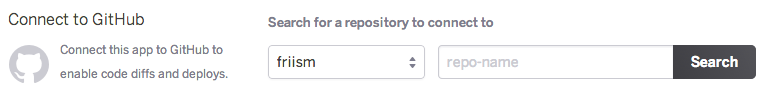
\includegraphics[scale=0.5]{deploy-github-dashboard.jpg}  
	\caption[Deploy menggunakan Github Dashboard]{Deploy menggunakan Github Dashboard} 
	\label{fig:deploy-github-dashboard} 
\end{figure}
Deploy dengan cara ini membuat Heroku dapat dengan otomatis melakukan deploy ke GitHub apabila build berhasil. Pengembang perlu mengaktifkan GitHub integration terlebih dahulu sebelum dapat melakukan deploy. Setelah itu, pengembang harus melakukan otentikasi dengan akun GitHub. Otentikasi ini hanya perlu dilakukan satu kali per satu akun Heroku. Setelah itu, pengembang dapat memilih repository yang ingin disambungkan dengan perangkat lunak Heroku (Gambar~\ref{fig:deploy-github-dashboard}).

\begin{figure}[H]
	\centering  
	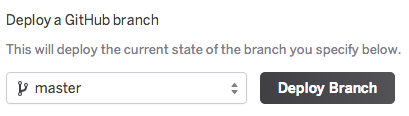
\includegraphics[scale=0.5]{deploy-github-manual.jpg}  
	\caption[Deploy menggunakan Github secara manual]{Deploy menggunakan Github secara manual} 
	\label{fig:deploy-github-manual} 
\end{figure}
\begin{figure}[H]
	\centering  
	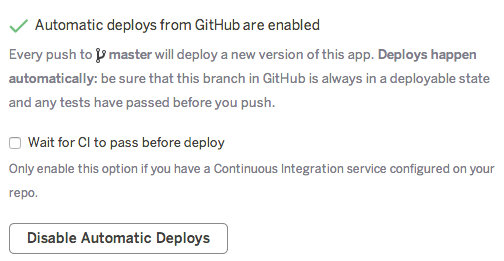
\includegraphics[scale=0.5]{deploy-github-automatic.jpg}  
	\caption[Deploy menggunakan Github secara otomatis]{Deploy menggunakan Github secara otomatis} 
	\label{fig:deploy-github-automatic} 
\end{figure}
Ada dua cara untuk melakukan deploy, yaitu secara manual dan secara otomatis. Untuk cara manual, pengembang melakukan deploy dari GitHub (Gambar~\ref{fig:deploy-github-manual}). Untuk cara otomatis, pengembang harus mengaktifkan "Automatic deploys from GitHub" (Gambar~\ref{fig:deploy-github-automatic}).

\subsubsection{Deploy Langsung di situs Heroku}
Tombol "Deploy to Heroku" memungkinkan pengguna untuk melakukan deploy perangkat lunak tanpa meninggalkan situs Heroku dan hampir tidak memerlukan konfigurasi. Penggunaan tombol ini ideal untuk pelanggan, dan pemelihara proyek yang bersifat open-source.
% Contoh tampilan tombol di Node.js app

Sebelum dapat melakukan deploy dengan cara ini, perangkat lunak harus memiliki dokumen \texttt{app.json} yang sah di direktori root, dan source code perangkat lunak harus berada di repository GitHub.

\texttt{app.json} adalah dokumen berisi deskripsi perangkat lunak web. Isinya dapat berupa environment variable, add-ons, dan informasi lain yang diperlukan untuk menjalankan perangkat lunak pada Heroku. Heroku tidak mewajibkan pengembang menuliskan informasi tertentu, tapi Heroku merekomendasikan untuk setidaknya menuliskan nama perangkat lunak(\texttt{name}), deskripsi perangkat lunak (\texttt{description}), dan logo perangkat lunak (\texttt{logo}). Berikut contoh isi dari \texttt{app.json} :
\begin{lstlisting}

{
  "name": "Node.js Sample",
  "description": "A barebones Node.js app using Express 4",
  "repository": "https://github.com/heroku/node-js-sample",
  "logo": "https://node-js-sample.herokuapp.com/node.png",
  "keywords": ["node", "express", "static"]
}

\end{lstlisting}

\subsection{Basis Data dan Manajemen Data}
Heroku menyediakan tiga layanan data untuk semua pelanggan :
\begin{itemize}
\item Heroku Postgres
\item Heroku Redis
\item Apache Kafka
\end{itemize}
Heroku juga menyediakan pilihan lain untuk pelanggan Heroku Enterprise, yaitu Heroku Connect. Selain itu, Heroku juga memungkinkan penggunaan layanan data dari pihak ketiga. Layanan data dari pihak ketiga ini tersedia sebagai add-ons.

\subsubsection{Heroku Postgres}
Heroku Postgres adalah basis data SQL yang disediakan secara langsung oleh Heroku. Heroku Postgres dapat diakses oleh bahasa apapun dengan PostgreSQL driver. Heroku secara otomatis menambahkan add-ons Heroku Postgres setiap perangkat lunak dibuat, sehingga pengembang tidak perlu menambahkannya secara manual. Namun, pengembang dapat menambahkannya secara manual, dengan mengetikkan perintah :
\begin{lstlisting}
	
	$ heroku addons:create heroku-postgresql:<PLAN_NAME>
	
\end{lstlisting}
<PLAN\_NAME> adalah tipe Heroku Postgres yang ingin dipakai. Heroku secara otomatis menggunakan Heroku Postgres tipe \texttt{hobby-dev}.

Heroku Postgres memiliki lima tipe Heroku Postgres :
\begin{itemize}
\item Hobby Tier : untuk perangkat lunak dengan toleransi gagal bekerja sampai 4 jam per bulan.
\item Standard Tier : untuk perangkat lunak dengan toleransi gagal bekerja sampai 1 jam per bulan.
\item Premium Tier : untuk perangkat lunak dengan toleransi gagal bekerja sampai 15 menit per bulan.
\item Private Tier : untuk pengguna Heroku Enterprise, memiliki toleransi gagal bekerja sampai 15 menit per bulan.
\item Shield Tier : untuk pengguna Heroku Enterprise yang menginginkan basis data yang compliance-capable, memiliki toleransi gagal bekerja sampai 15 menit per bulan.
\end{itemize}
Selain tipe Hobby, basis data memiliki fitur fork, follow, rollback, dan Disk Encryption. Hanya tipe Hobby yang gratis.

Pengembang juga dapat menambahkan versi yang ingin dipakai dengan cara menambahkan \texttt{--version} di belakang perintah tersebut, contoh :
\begin{lstlisting}
	
	$ heroku addons:create heroku-postgresql:<PLAN_NAME--version=9.5
	
\end{lstlisting}
Secara otomatis, Heroku menggunakan versi paling baru dari Heroku Postgres. Saat skripsi ini ditulis, versi terbaru adalah versi 10.

Setelah dipasang, Heroku akan secara otomatis menambahkan config var \texttt{DATABASE\_URL} ke perangkat lunak. Apabila Heroku Postgres yang dipakai ada lebih dari satu, nama config var akan menjadi \texttt{HEROKU\_POSTGRESQL\_<COLOR>\_URL} dengan <COLOR> adalah nama warna yang dihasilkan secara acak. Contoh : \texttt{HEROKU\_POSTGRESQL\_<BLUE>\_URL}.

Apabila pengembang menggunakan lebih dari satu basis data, pengembang dapat mengatur basis data utama. Basis data utama dapat diatur dengan perintah :
\begin{lstlisting}
	
	$ heroku pg:promote <database_url>
	
\end{lstlisting}
<PLAN\_NAME> adalah tipe Heroku Redis yang ingin dipakai. Heroku Redis memiliki dua tipe : Hobby Dev dan Premium. Hobby Dev gratis, sedangkan Premium berbayar. Perbedaannya terletak pada jumlah memori dan batas koneksi yang dapat dibuat.

Heroku Redis memiliki kelebihan sebagai berikut :
\begin{itemize}
\item Memiliki analisa performa yang dapat membantu menemukan masalah basis data dengan mudah
\item Heroku dapat diskala sesuai kebutuhan memori dan koneksi.
\end{itemize}



\subsubsection{Heroku Redis}
Heroku Redis adalah basis data berbasis key-value store yang bersifat in-memory. Heroku dijalankan oleh Heroku dan dikelola sebagai add-on Heroku Redis dapat diakses oleh bahasa apapun dengan Redis driver. Cara memasang add-on Heroku Redis :
\begin{lstlisting}
	
	$ heroku addons:create heroku-redis: <PLAN_NAME>
	
\end{lstlisting}

\subsubsection{Apache Kafka}
Apache Kafka adalah salah satu add-on di Heroku yang disediakan oleh Kafka yang berintegrasi penuh dengan Heroku. Apache Kafka dideskripsikan Kafka dideskripsikan oleh Heroku sebagai add-on yang memungkinkan pengembang mendistribusikan perangkat lunak yang dapat menangani jutaan event dan miliaran transaksi. Kafka didesain untuk memindahkan ephemeral data yang sangat besar dengan reliabilitas yang tinggi dan toleran akan kerusakan.

Pengembang harus memasang Python 2.7, node 8.x, .NET Framework, dan Visual C++ Build Tools terlebih dahulu sebelum memasang Apache Kafka. Setelah itu, pengembang mengetikkan perintah :
\begin{lstlisting}
	
	$ heroku plugins:install heroku-kafka
	
\end{lstlisting}

%2.3 IMAP
\section{IMAP}
\label{sec:IMAP}
IMAP (Internet Message Access Protocol) adalah metode untuk mengakses pesan elektronik yang disimpan di sebuah mail server.
\subsection{PHP IMAP ~\cite{php-imap}}
Ekstensi ini dapat digunakan apabila c-client library sudah terpasang. Library ini dapat ditemukan di https://www.washington.edu/imap/. Dokumen IMAP tidak boleh diletakkan langsung ke dalam direktori system, karena dapat memicu konflik. Sebaiknya membuat direktori baru di dalam direktori system, lalu memasukkan dokumen IMAP ke dalamnya. Contoh : \texttt{/usr/local/imap-2000b}. Di dalam direktori baru tamabahkan direktori lagi bernama \texttt{lib/} dan \texttt{include/}. Semua dokumen dengan ekstensi \texttt{.c} dimasukkan ke direktori \texttt{lib/}. Saat IMAP dikompilasi, dokumen bernama \texttt{c-client.a} akan terbentuk. Dokumen tersebut juga diletakkan di direktori \texttt{lib/}.

Setelah itu, kompilasi PHP dengan --with-imap[=DIR]. DIR disini adalah tempat c-client. Contoh : \texttt{with-imap=/usr/local/imap-2000b}. Pengguna sistem operasi Windows mungkin harus mengaktifkan \texttt{php\_imap.dll}.

IMAP tidak didukung pada sistem operasi Windows yang versinya lebih lama dari Windows 2000. Hal ini karena IMAP menggunakan fungsi enkripsi agar koneksi lewat SSL ke mail server aktif.

Di dalam sistem operasi Ubuntu, pemasangan PHP IMAP bisa dilakukan dengan mudah.
\begin{lstlisting}
	
	// Pasang libc-client-dev
	$ sudo apt-get install libc-client-dev

	// Pasang PHP<versi> imap:
	// sudo apt-get install php<versi>-imap
	// Contoh : 
	sudo apt-get install php5-imap
		
\end{lstlisting}

%%2.4 Line@.
%\section{Line@}
%\label{sec:Line@}
%Line@ adalah layanan oleh LINE yang didesain khusus untuk bisnis atau organisasi. Line@ menyediakan berbagai fitur untuk mempromosikan suatu perusahaan, merek, atau produk dalam cara yang baru dan dengan jangkauan yang luas. Salah satu fitur tersebut adalah fitur "Message Broadcasts". Fitur ini memungkinkan pengguna mengirimkan pesan melalui perangkat lunak mobile LINE@ atau melalui perangkat lunak komputer LINE@ Manager dan menyebarkannya ke pelanggan dan fans yang telah menjadikan akun pengguna sebagai teman. LINE@ menawarkan beberapa fitur bawaan yang bisa digunakan di pesan, seperti kupon dan survei. Fitur "1-on-1 chat" memungkinkan pengguna membalas secara langsung pesan yang dikirimkan pelanggan dan fans yang menjadikan pengguna teman. Fitur "Timeline Posts" memungkinkan pengguna mengirimkan postingan di linimasa. Postingan tersebut bisa diberi "like" atau dikomentari sehingga dapat memaksimalkan potensi linimasi sebagai media pemasaran.

%2.4 Line
\section{Line}
\label{sec:Line}
Line adalah perangkat lunak pengirim pesan yang tersedia dalam platform android, ios, dan desktop. Line memiliki beberapa produk yang dapat digunakan pengembang perangkat lunak. Produk-produk tersebut adalah :
\begin{enumerate}
\item LINE Login

LINE Login adalah produk dari LINE yang memungkinkan pengembang membua perangkat lunaknya menyediakan pilihan masuk melalui akun LINE.

\item Messaging API

Messaging API adalah produk LINE yang memungkinkan pengembang untuk membangun bot sebagai sarana komunikasi dua arah antara layanan yang dibangun pengembang dengan pengguna LINE. Dengan Messaging API, pengembang dapat mengirimkan push message dan reply message. Push message adalahh pesan yang bot kirimkan ke pengguna LINE. Reply message adalah pesan yang bot kirimkan untuk membalas pesan dari pengguna LINE.

%messaging-api-push-reply-message.png

\item LINE Bot Designer

LINE Bot Designer adalah produk LINE yang memungkinkan pengembang membuat prototipe LINE bot lebih cepat dan lebih mudah tanpa mengetahui pemrograman. Dengan produk ini, pengembang dapat mendesain chatbots sesuai skenario yang diinginkan.

%bot-designer.png

\item Clova

Clova adalah sebuah AI Assistant (perangkat lunak dengan kecerdasan buatan yang berfungsi sebagai asisten) yang dipasang di dalam Clova Wave dan Clova Friends. Clova masih dalam tahap pengembangan dan (pada saat skripsi ini dibuat) tersedia dalam versi beta. Tidak ada dokumentasi resmi untuk produk ini, namun disediakan situs web untuk menggali informasi tentang Clova : https://clova-developers.line.me. Pada saat skripsi ini ditulis, situs web ini hanya tersedia dalam bahasa Jepang sehingga membutuhkan penerjemah apabila tidak menguasai bahasa Jepang.

% clova_site.png

\item LINE Pay

LINE Pay adalah produk LINE yang memungkinkan pengembang mengintegrasikan perangkat lunak yang dibuat pengembang dengan fitur pembayaran melalui LINE Pay. Pada saat skripsi ini dibuat, tidak ada dokumentasi resmi untuk mengintegrasikan LINE Pay dengan perangkat lunak yang pengembang buat. Namun, pengembang dapat menggali informasi tentang fitur LINE Pay di situs https://pay.line.me. Situs ini menyediakan informasi LINE Pay di negara Jepang, Republik Tiongkok / Taiwan, dan Thailand. Situs ini tersedia dalam bahasa Jepang, Korea, Inggris, China dengan aksara sederhana, China dengan aksara tradisional, dan Thailand.

% line_pay_site.png

\end{enumerate}

Di antara produk-produk yang disediakan LINE, penulis menggunakan Messaging API untuk mengirimkan notifikasi melalui LINE@.

\subsection{Messaging API } %~\cite{https://developers.line.me/en/docs/}
Line Menyediakan Messaging API untuk membangun messaging bot. Messaging API memungkinkan data dioper antara server dari perangkat lunak bot dengan LINE Platform. Ketika pengguna Line mengirimkan pesan ke bot, sebuah webhook akan terpicu dan LINE Platform akan mengirimkan permintaan ke URL webhook bot. Server akan mengirim permintaan ke LINE Platform untuk merespon pengguna. Permintaan akan dikirimkan dalam format JSON. 

% Gambar messaging-api-architecture.png

Pengembang dapat melakukan hal-hal berikut dengan Messaging API :
\begin{itemize}
\item Mengirimkan reply message
\item Mengirimkan push message
\item Mengirimkan berbagai jenis pesan
\item Mendapatkan profil pengguna yang berinteraksi dengan bot
\item Bergabung dengan percakapan grup /group chats
\end{itemize}

Untuk menggunakan Messaging API, pengembang memerlukan akun LINE@. Messaging API juga dapat digunakan menggunakan akun resmi /official accounts. Akun resmi mendapatkan fitur tambahan untuk pengguna enterprise.

Untuk memulai membangun bot dengan Messaging API, pengembang perlu membuat channel terlebih dahulu. Channel adalah penyambung antara LINE platform dan perangkat lunak yang dibuat pengembang. Berikut langkah-langkah untuk membuat channel :
\begin{enumerate}
\item Langkah ke-1 : Masuk ke LINE Developers console

Pengembang perlu masuk ke LINE Developers console (https://developers.line.me/en/) dengan alamat email dan password dari akun LINE pengembang. Jika pengembang belum memiliki akun LINE, pengembang perlu mengunduh perangkat lunak LINE untuk mendaftar akun LINE.

% line-developers-console-login.png

\item Langkah ke-2 : Mendaftar sebagai developer (pengembang)

Apabila pengembang baru pertama kali masuk ke LINE Developers console, pengembang perlu membuat akun developer. Pengembang hanya perlu mencantumkan nama dan alamat email untuk mendaftar.

% line-developers-console-register-developer.png

\item Langkah ke-3 : Membuat provider baru

Provider adalah individu atau perusahaan yang menyediakan perangkat lunak yang akan dibuat. Pengembang perlu mencantumkan nama provider untuk membuat provider baru. Pengembang dapat menuliskan nama pengembang sendiri atau nama perusahaan pengembang.

% line-developers-console-create-provider.png

\item Langkah ke-4 : Membuat channel

Pengembang perlu memasukkan informasi yang dibutuhkan untuk membuat channel :
\begin{itemize}
\item Ikon perangkat lunak

Dokumen gambar untuk ikon perangkat lunak harus dibawah 3MB dengan ekstensi JPEG/PNG/GIF/BMP.

\item Nama perangkat lunak

Nama perangkat lunak tidak boleh lebih dari 20 karakter. Kata "LINE" tidak dapat digunakan sebagai nama perangkat lunak, walaupun kapitalisasinya tidak sama. Setelah dikonfirmasi, nama perangkat lunak tidak dapat diubah untuk tujuh hari ke depan.

\item Deskripsi perangkat lunak

Deskripsi perangkat lunak tidak boleh lebih dari 500 karakter.

\item Plan

Terdapat dua pilihan, Developer Trial dan Free. Plan Developer Trial memungkinkan pengembang untuk membuat bot yang dapat mengirimkan push message dan memiliki 50 teman. Apabila pengembang memilih plan ini, maka pengembang tidak dapat melakukan upgrade atau membeli ID premium. Plan Free memungkinkan pengembang untuk membuat bot dengan jumlah teman tak terbatas, namun pengembang tidak dapat mengirimkan push message. Pengembang dapat melakukan upgrade kapan saja dengan plan ini.

\item Kategori dan Subkategori

Pengembang dapat memilih kategori dan subkategori yang cocok dengan perangkat lunak yang sedang dikembangkan.

\item Alamat email

Alamat email yang dicantumkan adalah alamat email yang akan menerima notifikasi dan pengumuman penting dari LINE. Maksimal karakter pada alamat email adalah 100 karakter.

\end{itemize}
% line-developers-console-create-channel.png

\item Konfirmasi

Konfirmasi channel yang baru saja dibuat.

%line-developers-console-confirm-channel.png
\end{enumerate}

%Setelah membangun channel, 